\documentclass[aspectratio=169]{beamer}
\usepackage{./tex_refs/tomcom}

\usefonttheme{serif}

\title{Railway track fault detection}
\author{Tamás DEMUS}
\date{18\textsuperscript{th} of July 2023}

\begin{document}

\begin{frame}
    \thispagestyle{empty}
    \begin{columns}
        \begin{column}{0.4\textwidth}
            \begin{figure}[H]
                \raggedleft
                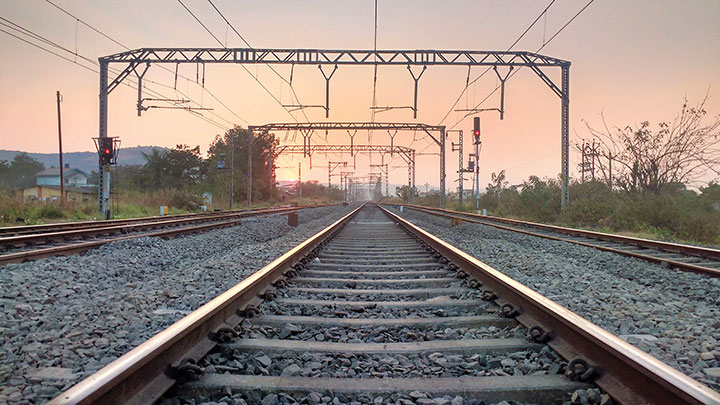
\includegraphics[width=\textwidth]{./tex_images/rail_track.jpg}
            \end{figure}
        \end{column}

        \begin{column}{0.5\textwidth}
            {\Large\textbf{Railway track fault detection}}

            with Artificial Intelligence

            \vspace*{0.5cm}
            \textbf{\textsc{Tamás Demus}}

            {\small 2023.07.18}
        \end{column}
    \end{columns}
\end{frame}

\begin{frame}{Motivation}
    \pause
    \begin{columns}[T]
        \begin{column}{0.3\textwidth}
            \begin{figure}[H]
                \raggedleft
                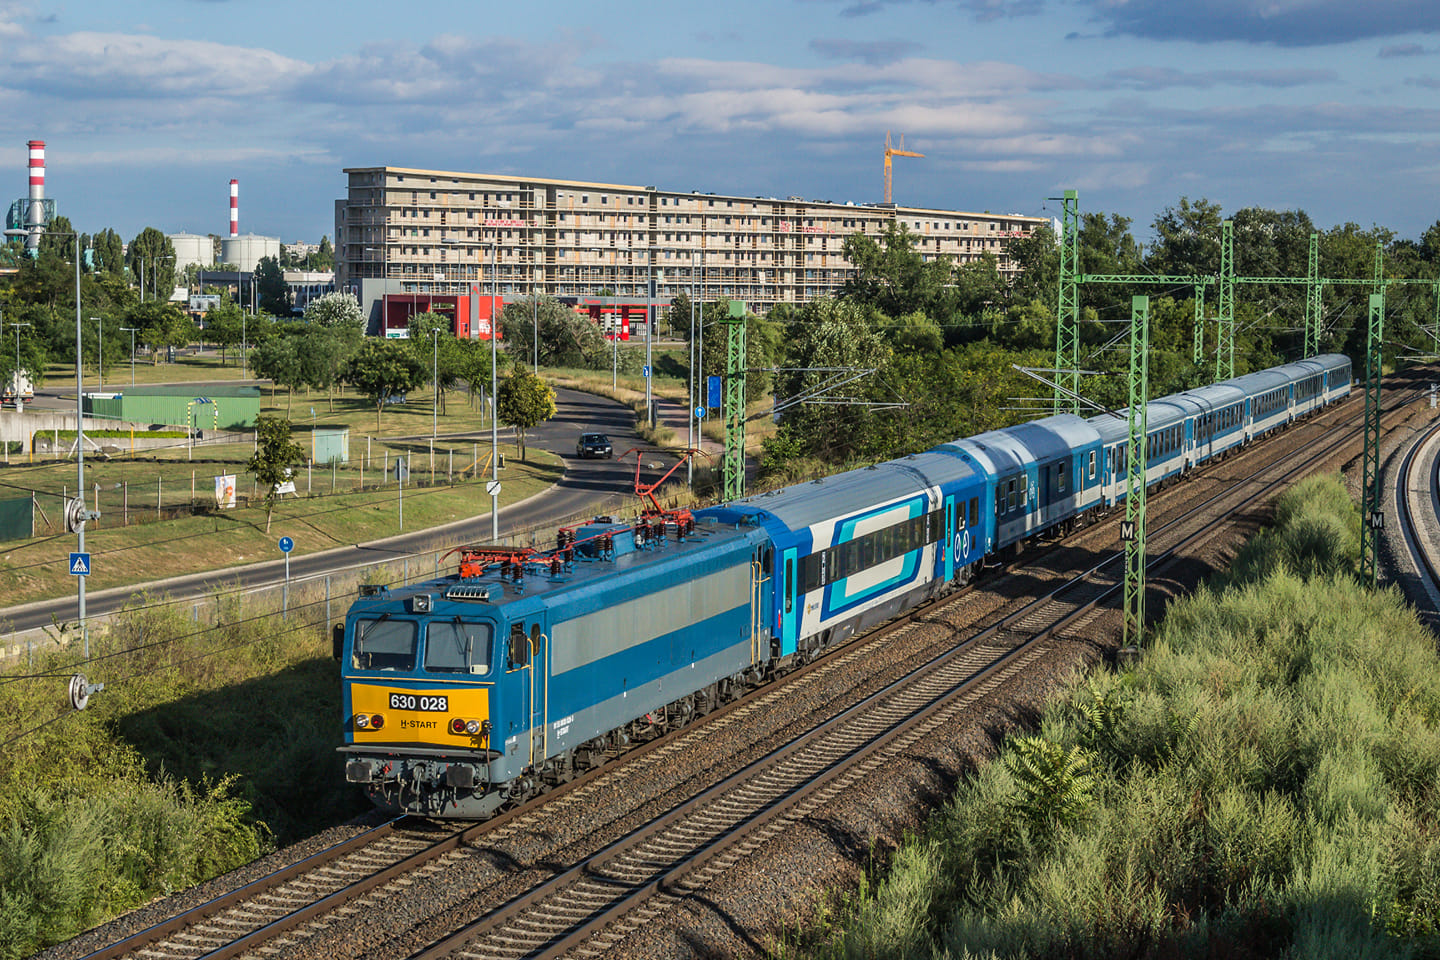
\includegraphics[width=0.9\textwidth]{./tex_images/gigant.jpg}
            \end{figure}
        \end{column}
        \begin{column}{0.65\textwidth}
            \vspace*{0.5cm}
            \begin{itemize}
                \item Interest in railway technology
                \item Desire for research
                \item Self education
            \end{itemize}
        \end{column}
    \end{columns}
    \pause

    \begin{columns}[T]
        \begin{column}{0.3\textwidth}
            \begin{figure}[H]
                \raggedleft
                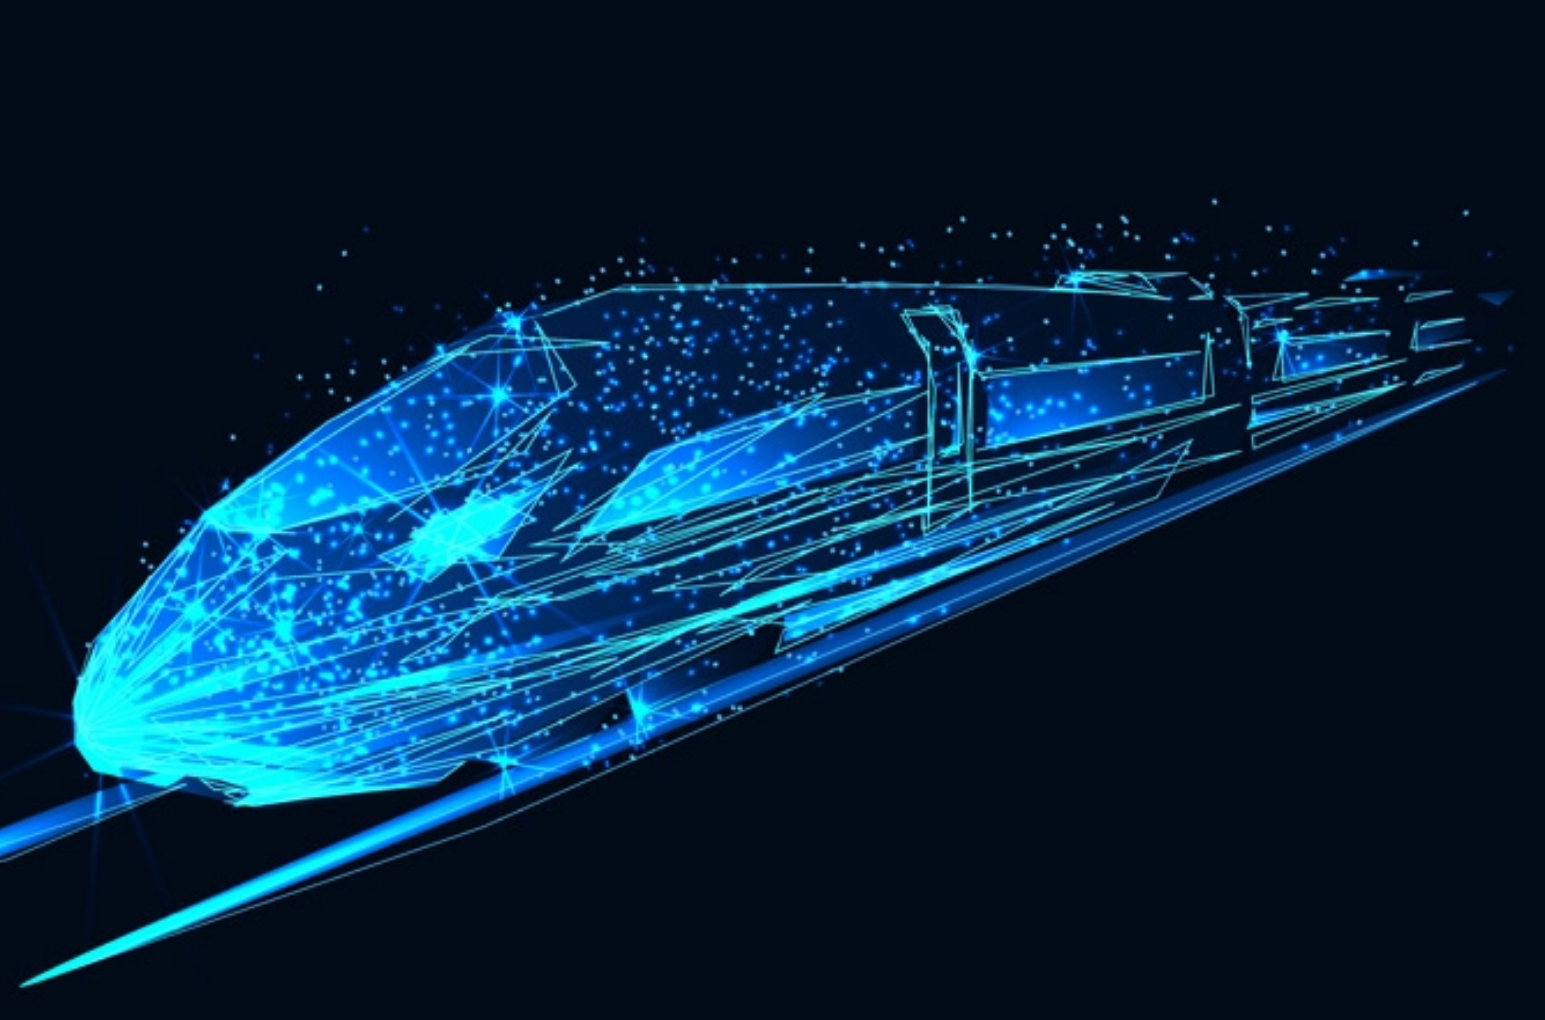
\includegraphics[width=0.9\textwidth]{./tex_images/digital_train.png}
            \end{figure}
        \end{column}
        \begin{column}{0.65\textwidth}
            \vspace*{0.5cm}
            \begin{itemize}
                \item Interest in computer science
                \item AI studies
            \end{itemize}
        \end{column}
    \end{columns}
\end{frame}

\begin{frame}{Available results}
    \pause
    \begin{columns}[T]
        \begin{column}{0.45\textwidth}
            Modelling practice
            \begin{itemize}
                \item Kaggle dataset
                \item Deep neural network
                \item Limited data quality and quantity
            \end{itemize}
        \end{column}
        \begin{column}{0.45\textwidth}
            \begin{figure}[H]
                \centering
                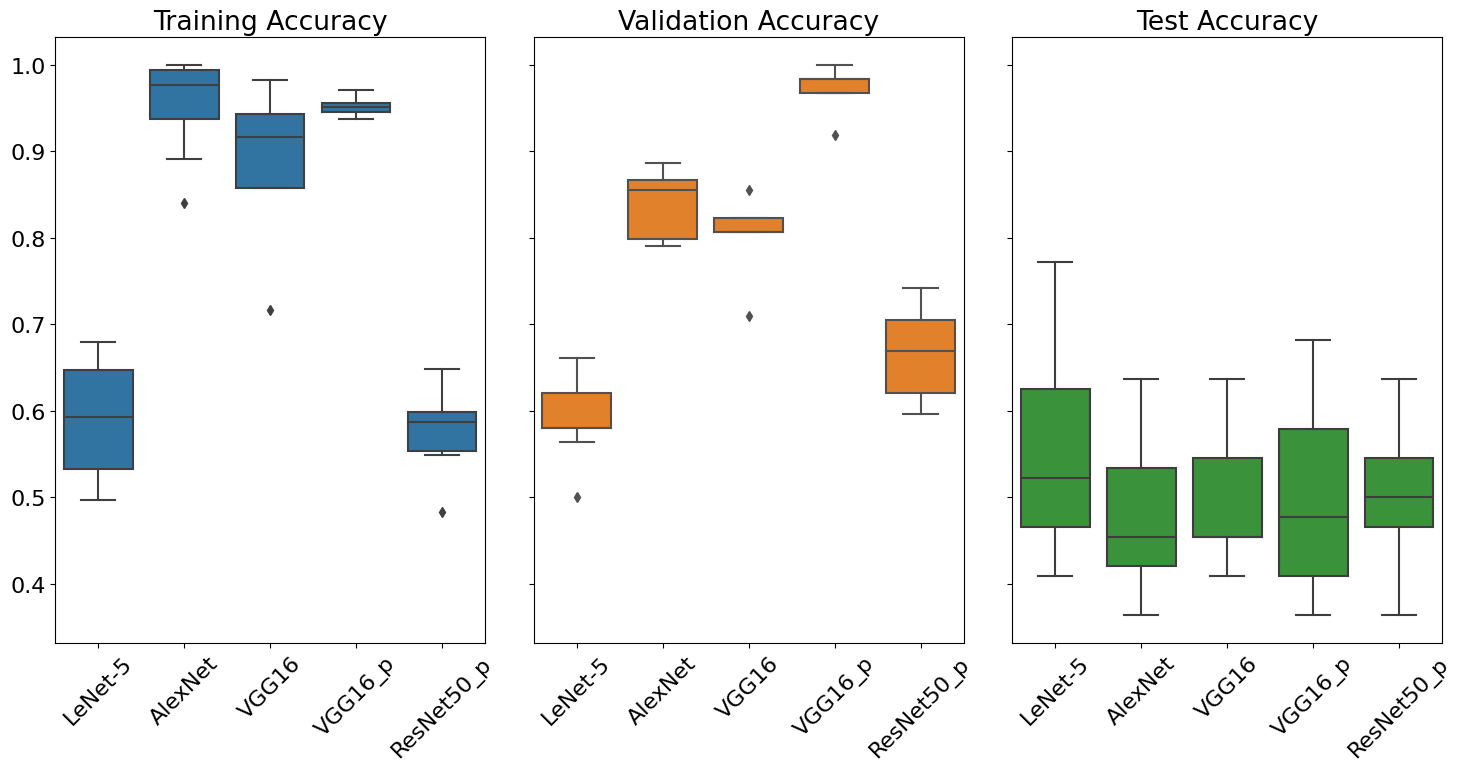
\includegraphics[height=0.4\textheight]{./tex_images/bootstrap_results.png}
            \end{figure}
        \end{column}
    \end{columns}
    \pause

    \begin{columns}[T]
        \begin{column}{0.45\textwidth}
            Thesis work
            \begin{itemize}
                \item Dataset from MÁV CRTI Ltd.
                \item Reconstruction of rail images
                \item Anomaly detection models
            \end{itemize}
        \end{column}
        \begin{column}{0.45\textwidth}
            \begin{figure}
                \centering
                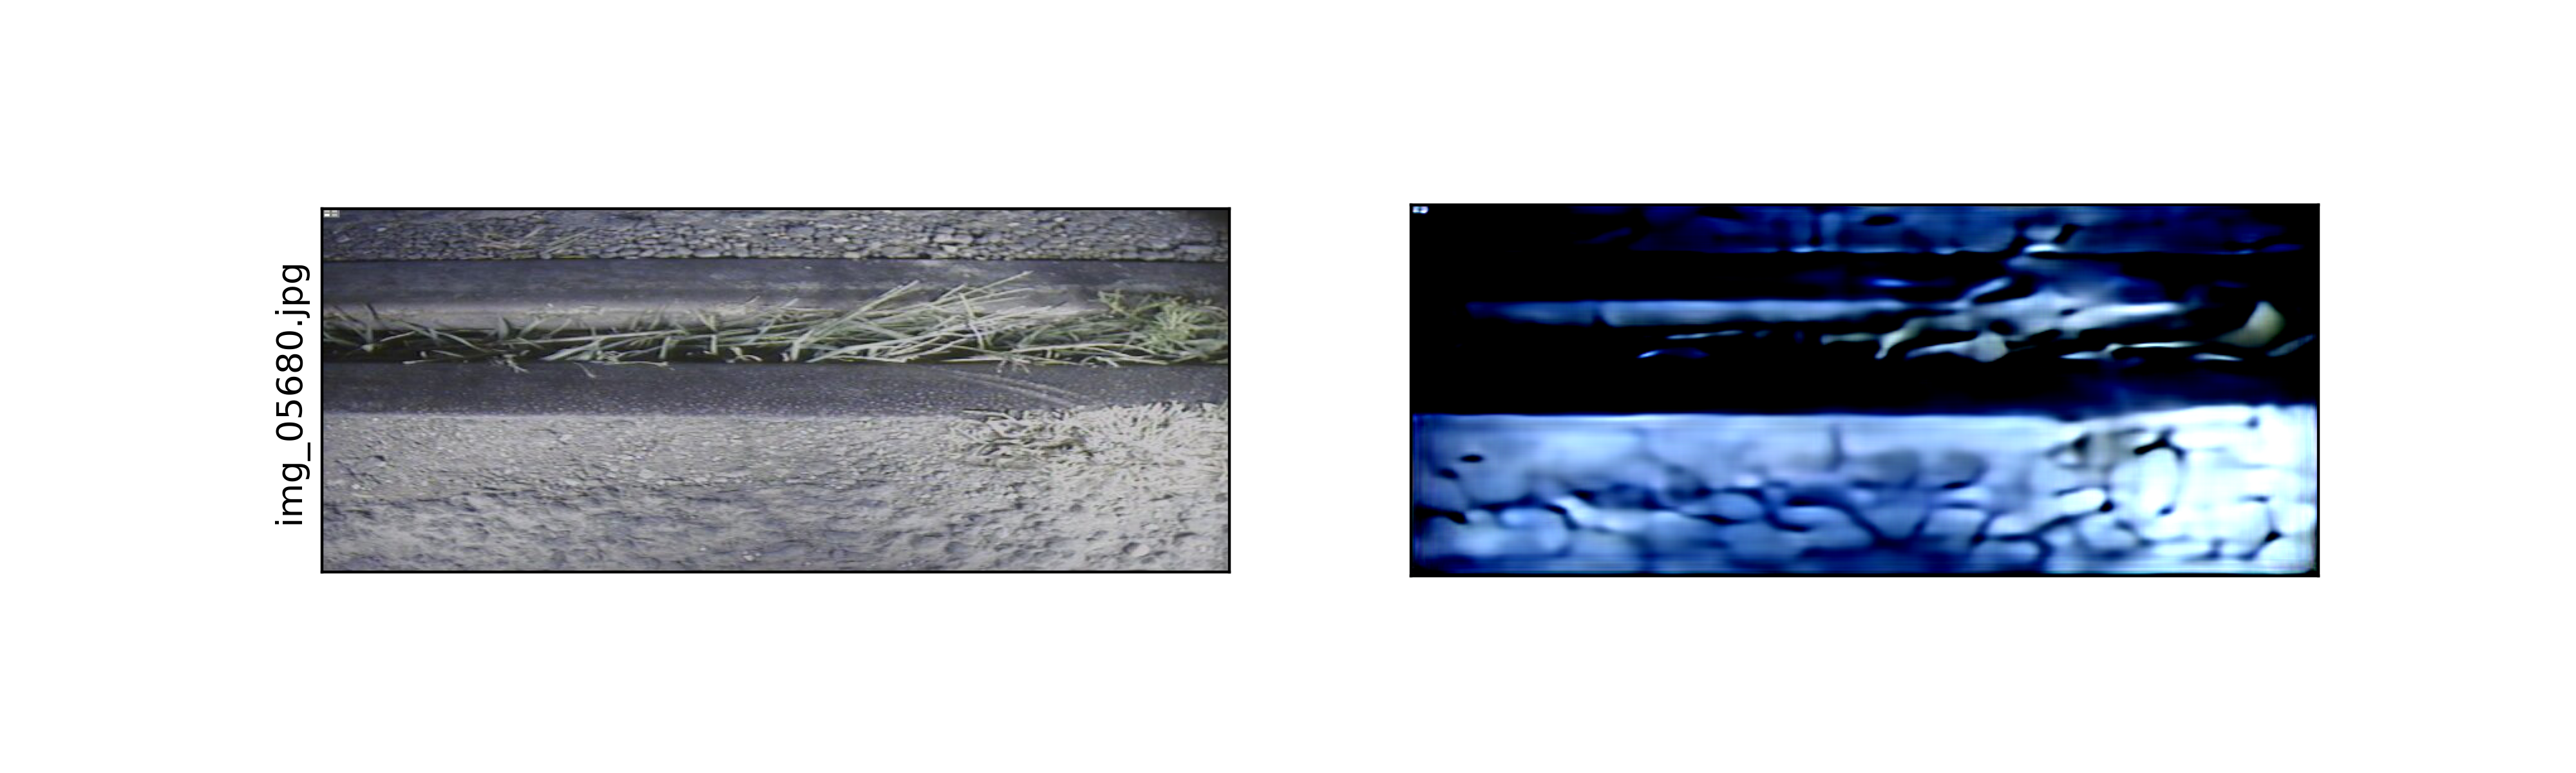
\includegraphics[width=\columnwidth,trim={0 1cm 0 1cm},clip]{./results/vgg19_vgg19/20230510_172958_predict_0.png}
            \end{figure}
        \end{column}
    \end{columns}
\end{frame}

\begin{frame}{Available results}
    \begin{figure}
        \centering
        \begin{subfigure}{0.3\textwidth}
            \centering
            \includegraphics[width=\textwidth]{./data/sd1_sample/normal/img_00006.jpg}
            \caption*{Normal rail}
        \end{subfigure}
        \begin{subfigure}{0.3\textwidth}
            \centering
            \includegraphics[width=\textwidth]{./data/sd1_sample/normal/img_00723.jpg}
            \caption*{Normal rail}
        \end{subfigure}
        \begin{subfigure}{0.3\textwidth}
            \centering
            \includegraphics[width=\textwidth]{./data/sd1_sample/normal/img_04857.jpg}
            \caption*{Normal rail}
        \end{subfigure}
        \begin{subfigure}{0.3\textwidth}
            \centering
            \includegraphics[width=\textwidth]{./data/sd1_sample/grass/img_05649.jpg}
            \caption*{Rails covered with grass}
        \end{subfigure}
        \begin{subfigure}{0.3\textwidth}
            \centering
            \includegraphics[width=\textwidth]{./data/sd1_sample/double_rail/img_05676.jpg}
            \caption*{Double rails}
        \end{subfigure}
    \end{figure}
\end{frame}

\begin{frame}{Available results}
    \begin{figure}
        \centering
        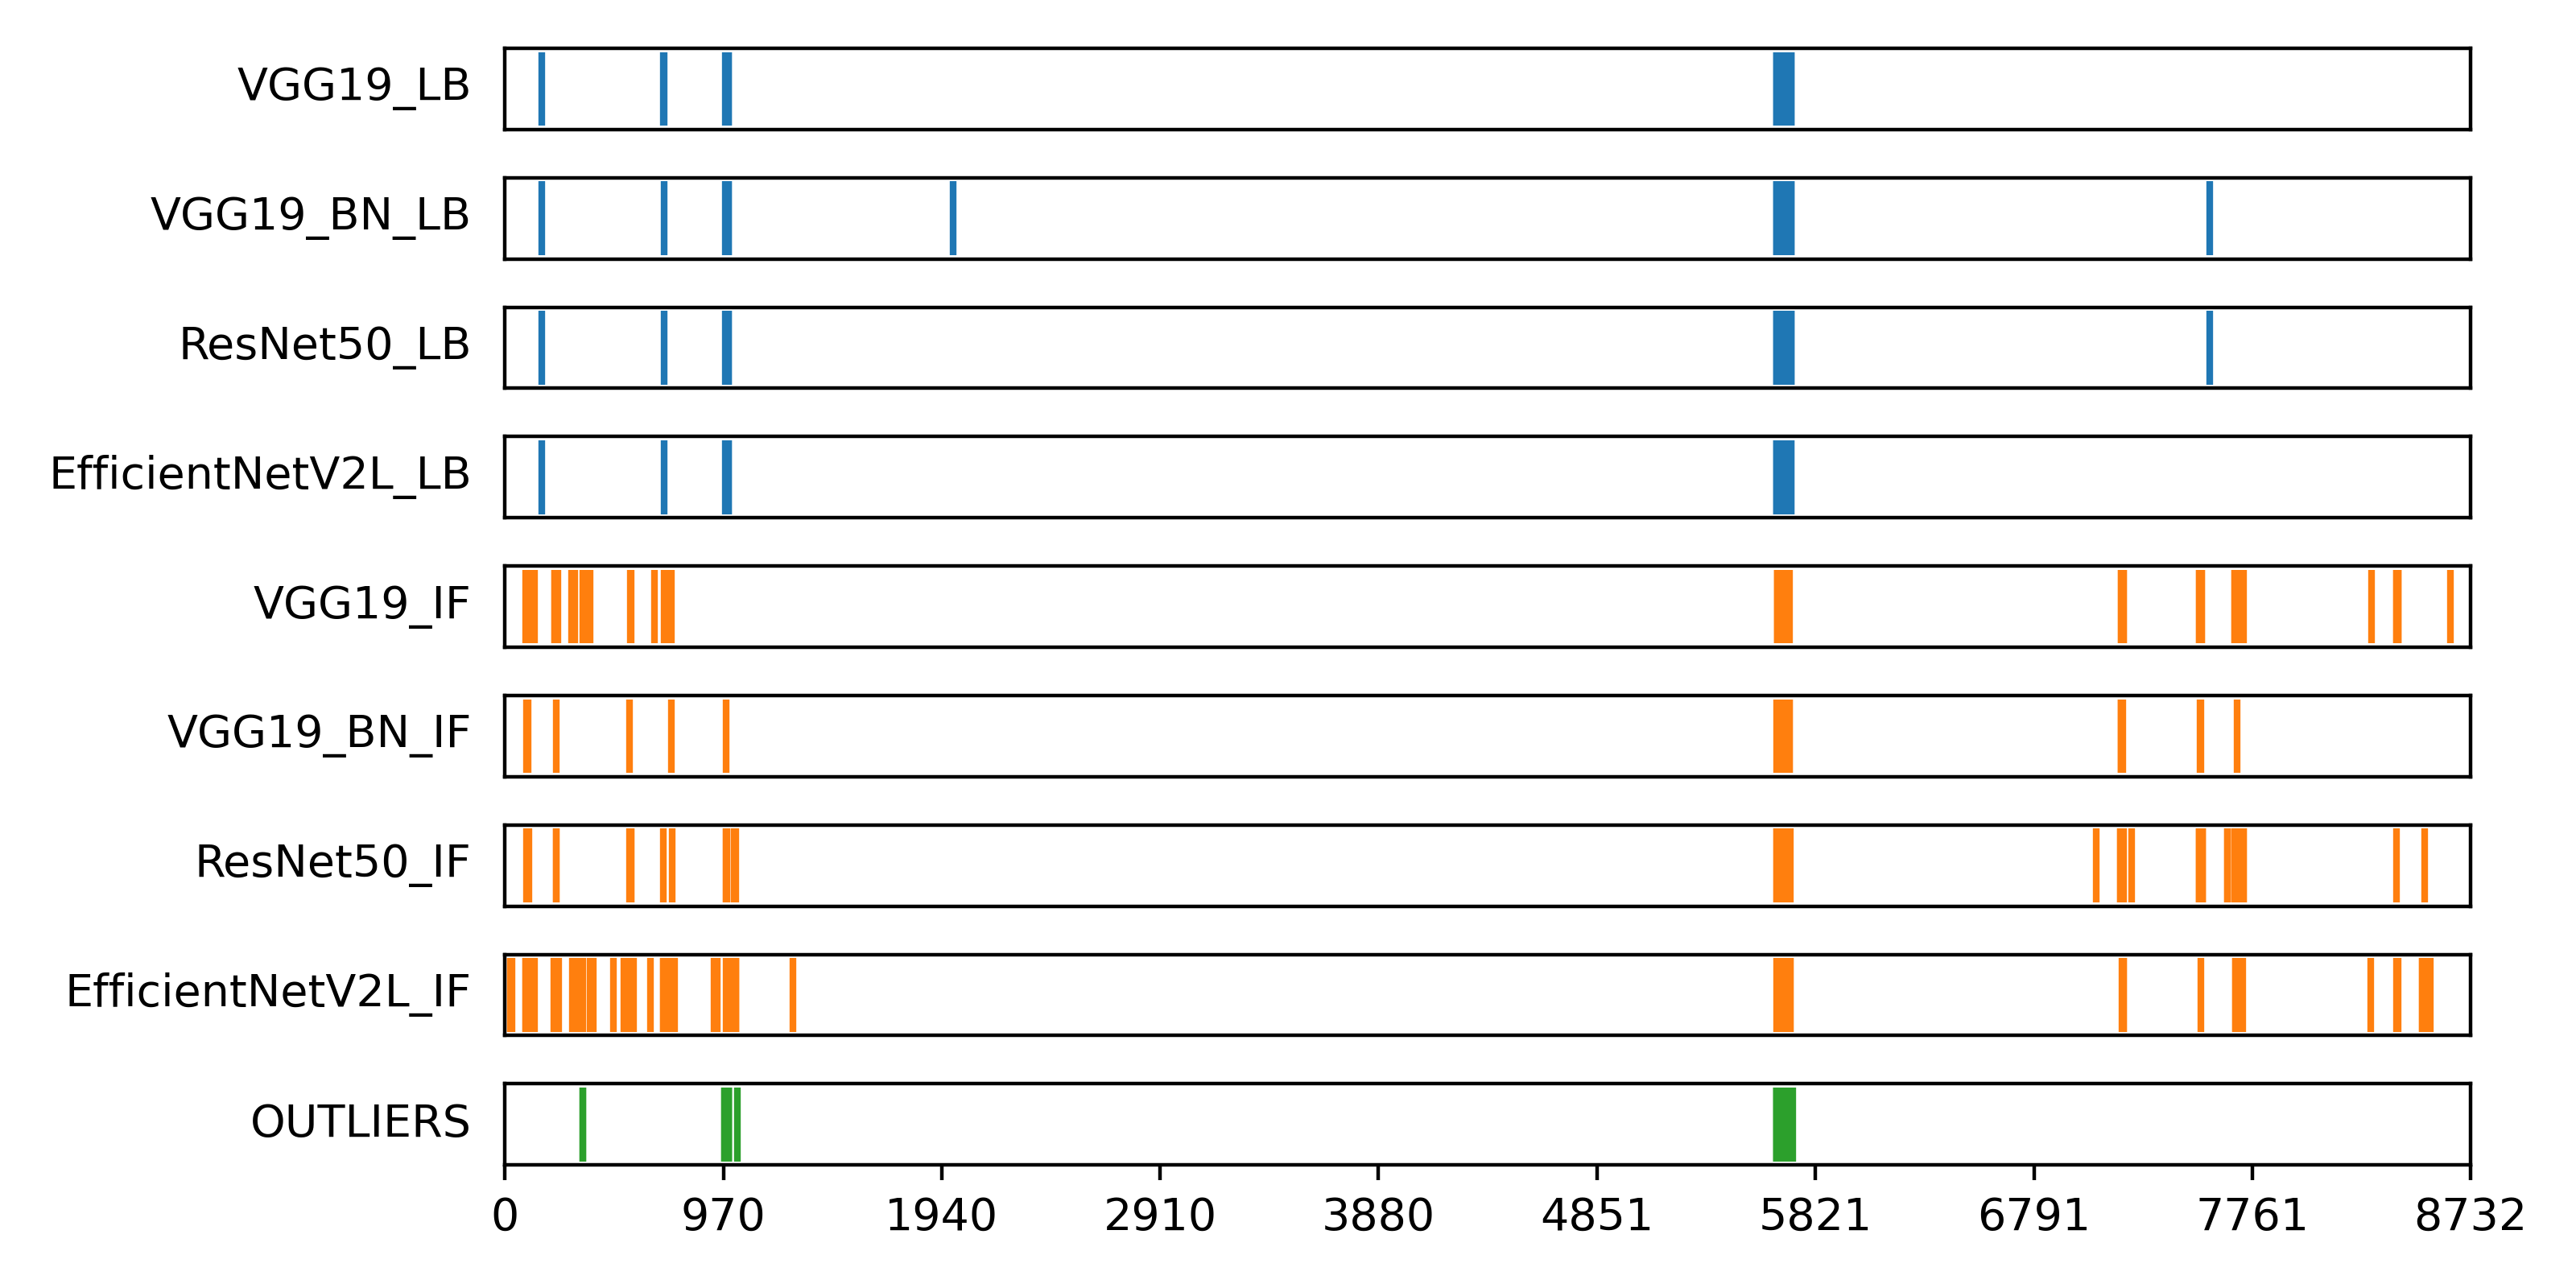
\includegraphics[width=0.9\textwidth]{./results/comparison/outlier_comparison.png}
    \end{figure}
\end{frame}

\begin{frame}{Next steps}
    \pause
    \begin{columns}[T]
        \begin{column}{0.3\textwidth}
            \begin{figure}[H]
                \centering
                
\includegraphics[width=0.6\textwidth]{./tex_images/mathai_alfa.jpg}
            \end{figure}
        \end{column}
        \begin{column}{0.65\textwidth}
            \vspace*{0.5cm}
            \begin{itemize}
                \item Further models and model improvements
                \item Scientific publications
                \item Research project
            \end{itemize}
        \end{column}
    \end{columns}
    \pause

    \begin{columns}[T]
        \begin{column}{0.3\textwidth}
            \begin{figure}[H]
                \centering
                
\includegraphics[width=0.5\textwidth]{./tex_images/mav_kfv_logo.jpeg}
            \end{figure}
        \end{column}
        \begin{column}{0.65\textwidth}
            \vspace*{0.5cm}
            \begin{itemize}
                \item Provides video footage from rail inspections
                \item Possible real life application
                \item Joint project work
            \end{itemize}
        \end{column}
    \end{columns}
\end{frame}

\begin{frame}{Motivation}
    \begin{columns}[T]
        \begin{column}{0.3\textwidth}
            \begin{figure}[H]
                \raggedleft
                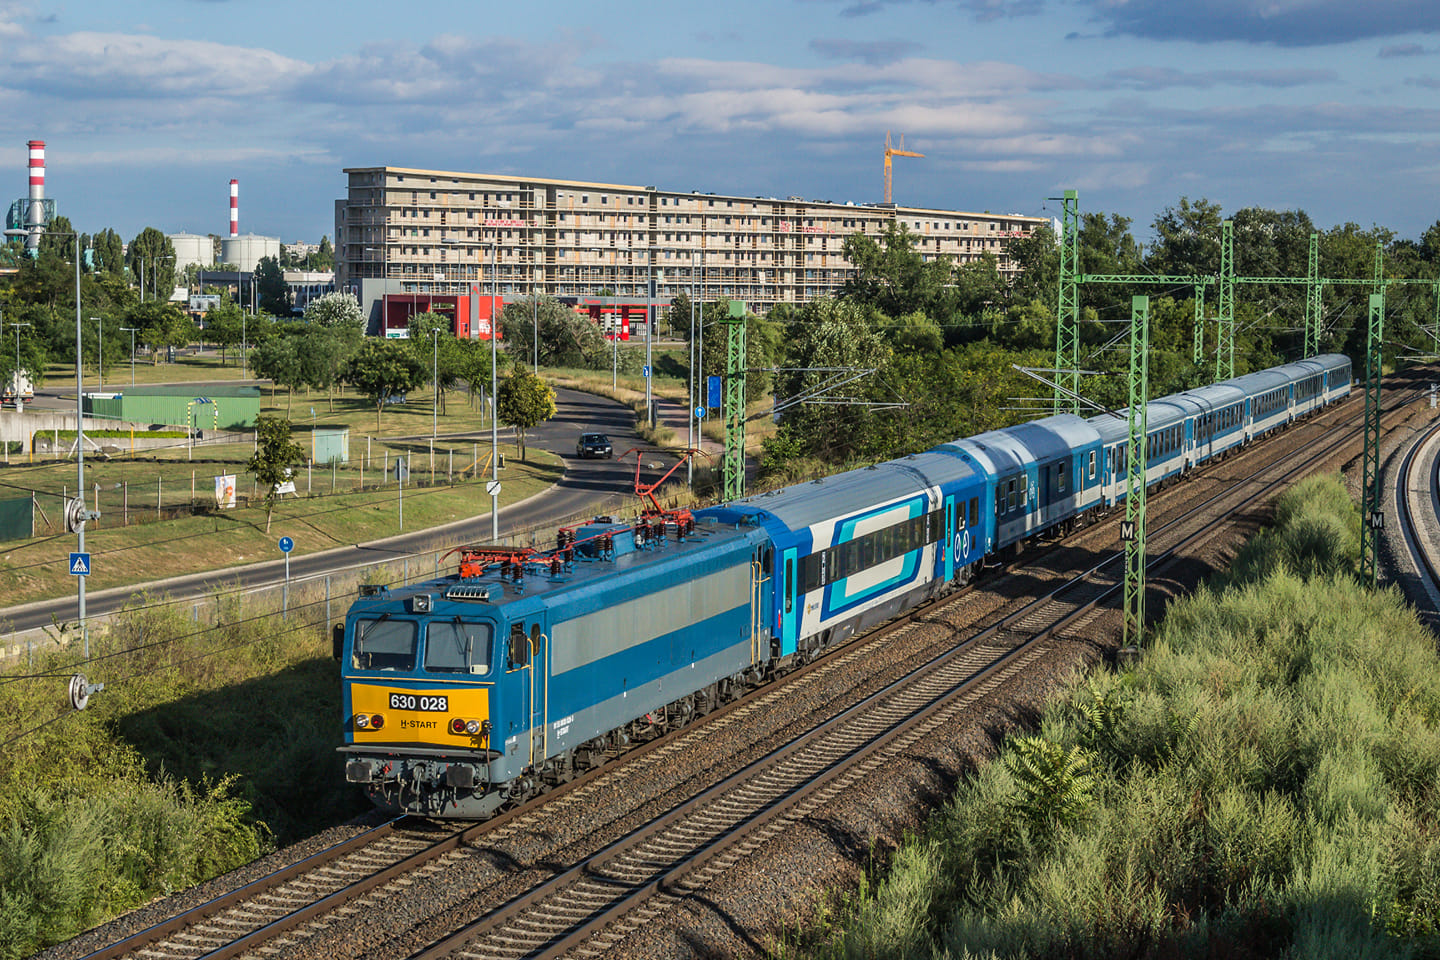
\includegraphics[width=0.9\textwidth]{./tex_images/gigant.jpg}
            \end{figure}
        \end{column}
        \begin{column}{0.65\textwidth}
            \vspace*{0.5cm}
            \begin{itemize}
                \item Interest in railway technology
                \item Desire for research
                \item Self education
                \item <2-> \alert{Scientific workshop}
            \end{itemize}
        \end{column}
    \end{columns}

    \begin{columns}[T]
        \begin{column}{0.3\textwidth}
            \begin{figure}[H]
                \raggedleft
                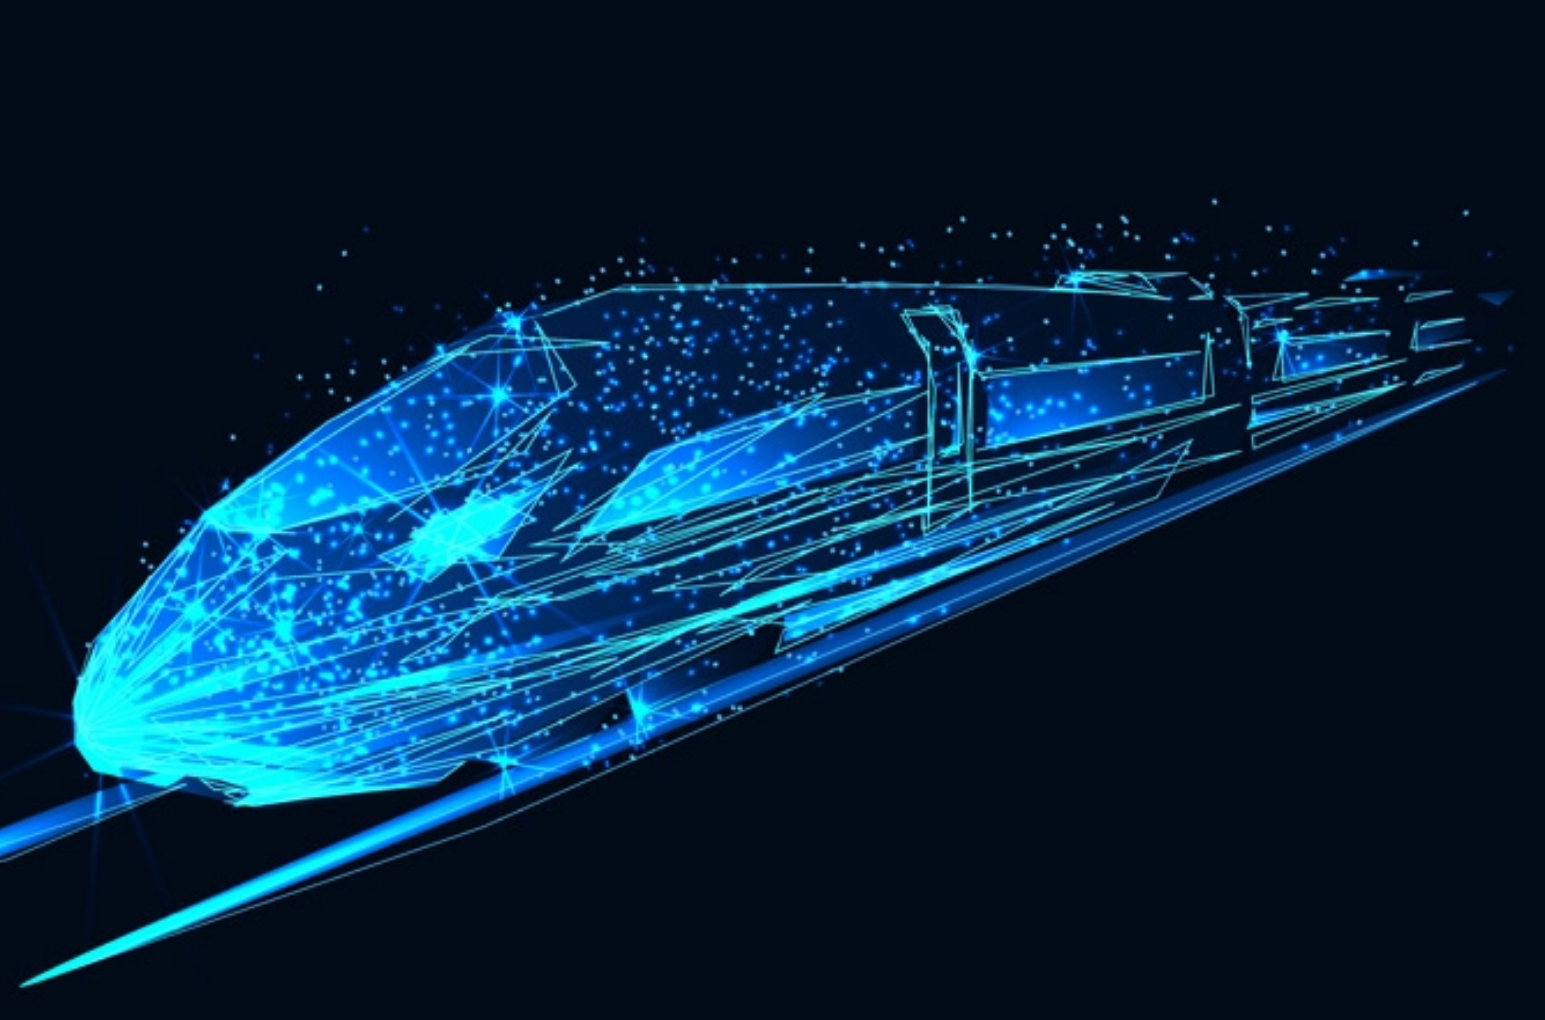
\includegraphics[width=0.9\textwidth]{./tex_images/digital_train.png}
            \end{figure}
        \end{column}
        \begin{column}{0.65\textwidth}
            \vspace*{0.5cm}
            \begin{itemize}
                \item Interest in computer science
                \item AI studies
                \item <3-> \alert{Research project}
                \item <4-> \alert{(Product development)}
            \end{itemize}
        \end{column}
    \end{columns}
\end{frame}

\begin{frame}{Next steps}
    \begin{columns}[b]
        \begin{column}{0.3\textwidth}
            \begin{figure}[H]
                \centering
                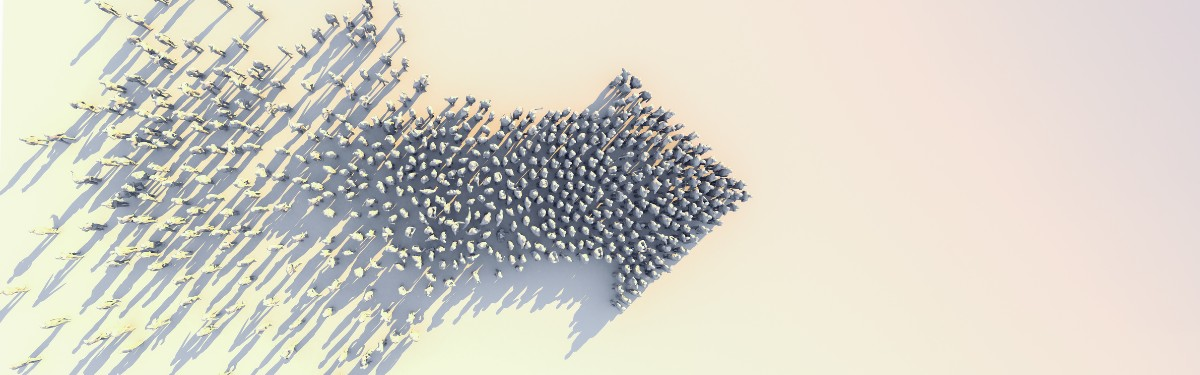
\includegraphics[width=\textwidth]{./tex_images/next_steps.jpg}
            \end{figure}
        \end{column}
        \begin{column}{0.65\textwidth}
            \vspace*{0.5cm}
            \begin{itemize}
                \item Identify project opportunities
                \item Assess scientific potential
                \item Search for contributors
            \end{itemize}
        \end{column}
    \end{columns}
    \vspace*{1cm}
    \pause

    \begin{columns}
        \begin{column}{0.3\textwidth}
            \begin{figure}[H]
                \centering
                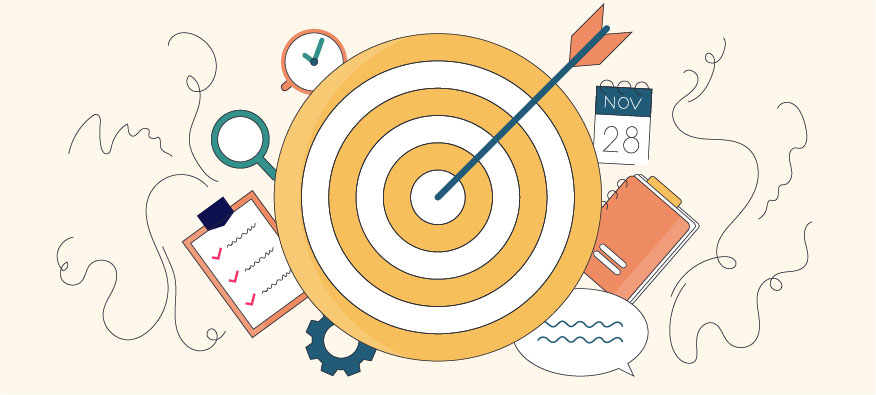
\includegraphics[width=\textwidth]{./tex_images/goal_setting.jpg}
            \end{figure}
        \end{column}
        \begin{column}{0.65\textwidth}
            \begin{itemize}
                \item Proof of concept
                      \begin{itemize}
                          \item Fit to MÁV CRTI Ltd. equipment
                          \item Limit failure type or location
                          \item Limit input data type (e.g.: no junctions)
                      \end{itemize}
                \item Outcome
                      \begin{itemize}
                          \item Research paper
                          \item Showcase
                      \end{itemize}
            \end{itemize}
        \end{column}
    \end{columns}
\end{frame}

\begin{frame}{Department of Highway and Railway Engineering}
    \pause
    \begin{columns}[T]
        \begin{column}{0.2\textwidth}
            Role
        \end{column}
        \begin{column}{0.7\textwidth}
            \begin{itemize}
                \item Center of Competence Railway Engineering
                \item Possible research contributor
            \end{itemize}
        \end{column}
    \end{columns}
    \vspace*{1cm}
    \pause

    \begin{columns}[T]
        \begin{column}{0.2\textwidth}
            Level of contribution
        \end{column}
        \begin{column}{0.7\textwidth}
            \begin{itemize}
                \item Consultation
                \item Literature research
                \item Scientific research
                \item Student support
            \end{itemize}
        \end{column}
    \end{columns}
\end{frame}

\begin{frame}{Form}
    \pause
    \begin{columns}[T]
        \begin{column}{0.2\textwidth}
            'Hobby'-project
        \end{column}
        \begin{column}{0.7\textwidth}
            \begin{itemize}
                \item Casual consultation
            \end{itemize}
        \end{column}
    \end{columns}
    \vspace*{1cm}
    \pause
    \begin{columns}[T]
        \begin{column}{0.2\textwidth}
            Informal project
        \end{column}
        \begin{column}{0.7\textwidth}
            \begin{itemize}
                \item Regular consultation
                \item Publications
                \item Case studies
            \end{itemize}
        \end{column}
    \end{columns}
    \vspace*{1cm}
    \pause
    \begin{columns}[T]
        \begin{column}{0.2\textwidth}
            Contractual form
        \end{column}
        \begin{column}{0.7\textwidth}
            \begin{itemize}
                \item Regular consultation
                \item Publications
                \item Case studies
                \item Proof of concept, Showcase
            \end{itemize}
        \end{column}
    \end{columns}
\end{frame}

\begin{frame}
    \thispagestyle{empty}
    \centering \Large
    Thank you very much for your kind attention!
\end{frame}

\end{document}